\chapter{Praxiseinsatz}
\label{cha:praxiseinsatz}

Dieses Kapitel beschreibt den praktischen Einsatz der Software und beleuchtet zudem einen bisher nicht diskutierten Aspekt der IT-Sicherheit.

\section{Anwendung}

Der Code der entwickelten Software wurde über ein GitHub-Repository\footnote{\url{https://github.com/Jomibe/ba}} veröffentlicht, sodass die Installation und Konfiguration des Bots für eine eigene Installation von Graylog wiederverwendet oder optimiert werden kann. Für den Betrieb ist es notwendig, zuvor die angeschlossenen Dienste inkl. der API-Zugriffsdaten zu konfigurieren. Im Anschluss kann die Software mit einem Python Interpreter ausgeführt werden und ist einsatzbereit, sobald die Vorbereitungsphase abgeschlossen ist. Mithilfe der aktivierten ausführlichen Ausgaben zum Programmablauf können die Vorgänge und dessen Auslöser gut zurückverfolgt werden. Im Folgenden zeigen zwei Abbildungen die Interaktion mit dem Bot über den Telegram Messenger:

\begin{figure}[h!]
    \centering
    \begin{minipage}{0.5\textwidth}
        \raggedright
        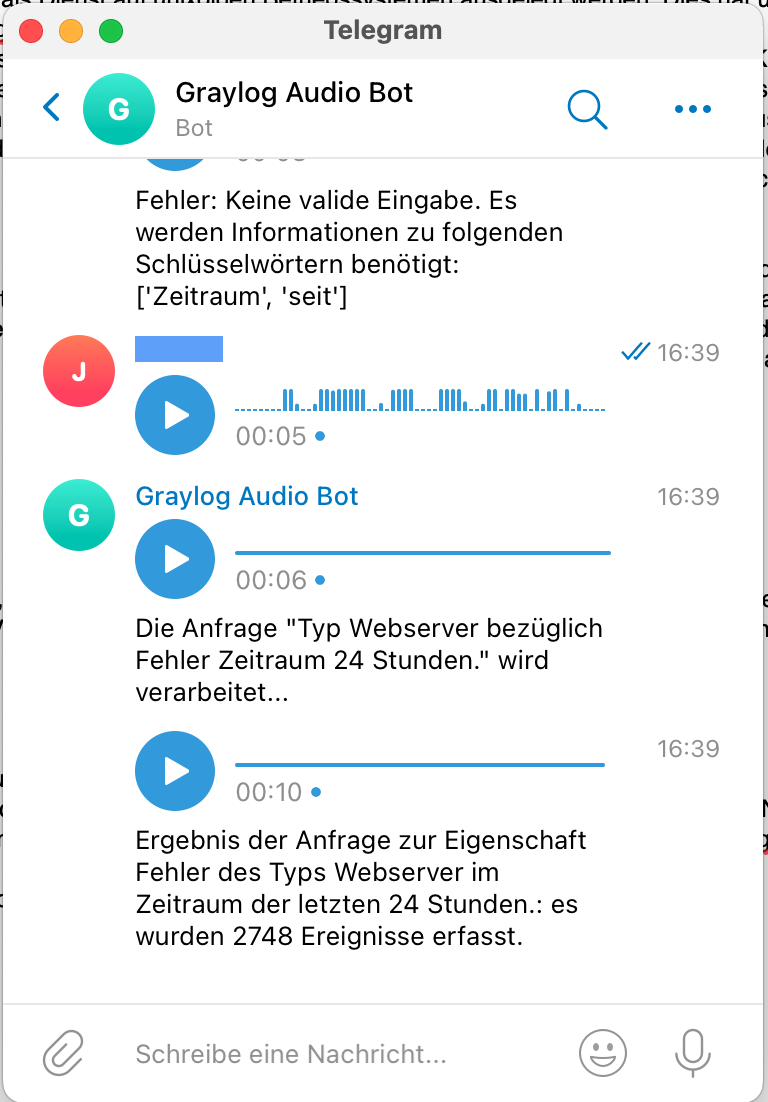
\includegraphics[width=0.9\textwidth]{bsp-betrieb}
        \caption{Bot beantwortet eine \\\hspace{\textwidth}Anfrage in Telegram.}
        \label{fig:bsp-betrieb}
    \end{minipage}\hfill
    \begin{minipage}{0.5\textwidth}
        \raggedleft
        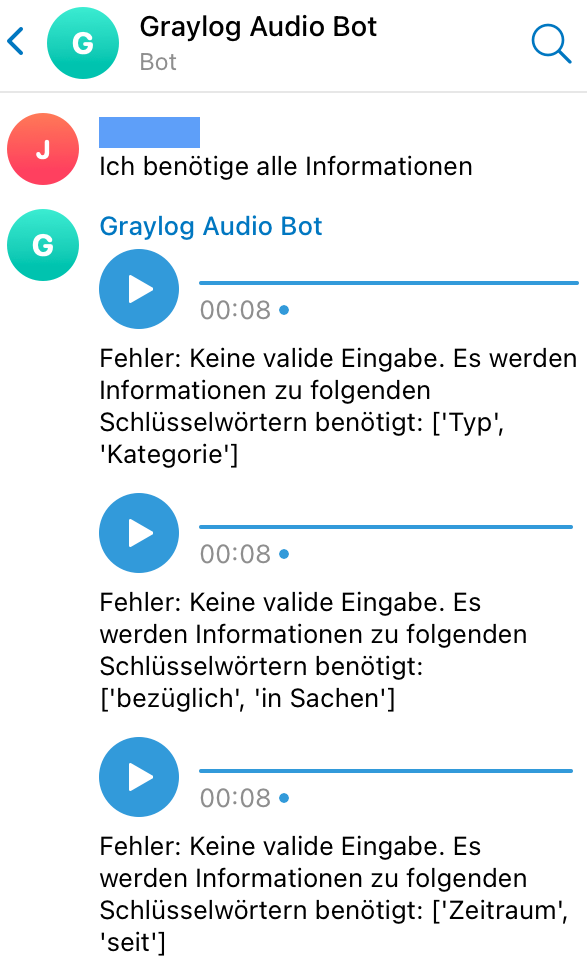
\includegraphics[width=0.9\textwidth]{bsp-fehler}
        \caption{Bot reagiert auf fehlerhafte \\\hspace{\textwidth}Anfrage in Telegram.}
        \label{fig:bsp-fehler}
    \end{minipage}
\end{figure}

Die \autoref{fig:bsp-betrieb} zeigt, wie der Bot eine Anfrage beantwortet. Zuerst wird dem Benutzer eine Rückmeldung gesendet, sobald die Transkription fertiggestellt ist. Im Anschluss erfolgt die Beantwortung der eingesendeten Anfrage. Alle Nachrichten des Bots werden in einer kombinierten Sprachnachricht gesendet, welche zusätzlich den gesprochenen Text in geschriebener Form enthält. Zusätzlich ist es möglich, Anfragen per Textnachricht einzusenden, wie \autoref{fig:bsp-fehler} zeigt:

In \autoref{fig:bsp-fehler} wurde dem Bot eine Nachricht zugestellt, welche nicht die erforderlichen Informationen beinhaltet. Der Bot prüft dies anhand der konfigurierten Schlüsselwörter und weißt den Anwender auf jede fehlende Information hin. 

\section{Qualitätskontrolle}

Nach Abschluss der Implementierung soll die Qualität der Software bezüglich der Benutzbarkeit im geplanten Anwendungsfall kurz erläutert werden. Die Qualität der Anwendung hängt stark von der Qualität der Spracherkennung ab, da hiervon die höchste Fehlerwahrscheinlichkeit ausgeht. Mit dem Vergleich verschiedener Dienste (vgl. \autoref{sec:vergleich-transkrip}) konnte dieses Qualitätsmerkmal bereits vor der Implementierung optimiert werden. Durch die Möglichkeit, Anfragen ebenfalls als Textnachricht an die Software zu übermitteln, kann der Anwender die Fehlerwahrscheinlichkeit bei der Erkennung des Anliegens reduzieren. Weiterhin ist es möglich, lokale Transkriptionsdienste, beispielsweise von der Tastatur-App auf einem Mobiltelefon zu nutzen. Ein weiteres Werkzeug für die Verbesserung der Spracherkennung sind die Aliasdefinitionen. Der Vergleich der verschiedenen Dienste hat bereits bei einer kleinen Stichprobe gezeigt, dass die Spracherkennung bei Fachbegriffen nicht verlässlich genug arbeitet. Die Definition von Begriffen aus der Alltagssprache als Alias für Fachbegriffe führt daher zu einer Verbesserung der Erkennungsquote und somit zu einem gesteigerten Qualitätsempfinden der Anwendung aus Sicht der Benutzer.

\section{IT-Sicherheit}

Aus Sicht der IT-Sicherheit bringt die Verwendung des Telegram-Bots Vorteile gegenüber der Verwendung der Graylog Webschnittstelle, sofern der Zugriff von außerhalb des Netzwerks erfolgt. Die Graylog-Instanz sammelt die Systemprotokolle sämtlicher Geräte im Netzwerk und ist damit ein besonders schützenswertes System in einem Firmennetzwerk. Der Zugriff von außerhalb sollte gut abgesichert werden. Es existieren mehrere Möglichkeiten, um webbasierte Systeme aus einem internen Netzwerk über das Internet erreichbar zu machen. Eine simple Möglichkeit besteht darin, auf dem Internetrouter eine Portweiterleitung einzurichten. Besser ist jedoch eine Veröffentlichung über einen 'Reverse Proxy'. Ein Proxy ist ein System, welches stellvertretend für ein weiteres System eine Kommunikation mit dem gewünschten Partner übernimmt. Häufig werden Proxys in Firmennetzwerken für die Filterung von besuchten Internetseiten eingesetzt. Dabei wendet sich ein PC im internen Netzwerk an den Proxyserver und fragt eine Internetressource an. Der Proxy agiert als Vermittler und bezieht die Internetressource, bevor er diese an den PC weiterleitet. Bei einem Reverse Proxy ist das Prinzip umgekehrt. Hier übernimmt der Vermittler die Kommunikation von Geräten außerhalb eines Netzwerks (beispielsweise dem Internet) stellvertretend für die Quelle und kontaktiert den gewünschten Verbindungspartner im internen Netzwerk. Der Vorteil eines Reverse Proxys gegenüber einer Portweiterleitung besteht darin, dass die HTTP-Anfragen detailliert bearbeitet, gefiltert und protokolliert werden können. Bestimmte Adressmuster, welche für Angriffe verwendet werden können so beispielsweise direkt blockiert werden. Der alleinige Einsatz eines Reverse Proxys mit Filter für die Veröffentlichung über das Internet reicht bei einem schützenswerten System nicht aus. Daher wird häufig eine HTTP-Authentifizierung zwischengeschaltet, welche durch die Anforderung von vom Ziel unabhängigen Zugangsdaten eine zusätzliche Sicherheitsebene schafft. Ein Reverse Proxy mit auf die Zielapplikation abgestimmten Filtermechanismen sowie einer zusätzlichen Authentifizierungsschicht bietet ausreichenden Schutz für eine Veröffentlichung im Internet. Der Einsatz eines solchen Reverse Proxies mit Graylog ist jedoch nicht möglich, da Graylog nicht kompatibel zu Anfragen mit HTTP-Authentifizierung ist\footnote{Fehlerbericht und Erweiterungsvorschlag eines Anwenders, welcher Graylog über einen Reverse Proxy mit HTTP-Authentifizierung erreichbar machen möchte: \url{https://github.com/Graylog2/graylog2-server/issues/6831}}. Eine Alternative zum Reverse Proxy bietet ein Dienst, welcher die Funktion eines Proxys oder Stellvertreters für die Verbindung zur Graylog-Webschnittstelle schafft. Dieser Dienst kann für beliebige Funktionen implementiert werden, welche über die Graylog REST-API Daten beziehen und weiterverarbeiten. Die in dieser Abschlussarbeit implementierte Software ist ein Beispiel für einen solchen Vermittler auf Applikationsebene \cite[S. 12 ff.]{bsi-websec}.
